\documentclass[a4paper,10pt]{article}
\usepackage[T1]{fontenc}
\usepackage{mathpazo}
\usepackage{tgpagella}
\usepackage[a4paper,margin=1.5cm]{geometry}
\usepackage{enumitem}
\usepackage[table]{xcolor}
\usepackage{array}
\usepackage{graphicx}
\usepackage{framed}
\usepackage[normalem]{ulem}
\usepackage{tikz}
\usetikzlibrary{arrows.meta, fit}
\definecolor{sectionshade1}{HTML}{23373B}
\definecolor{sectionshade2}{HTML}{2B4A4F}
\definecolor{sectionshade3}{HTML}{345E63}
\definecolor{sectionshade4}{HTML}{3D7278}
\definecolor{permaculturegreen}{HTML}{1FA32A}
\definecolor{scienceblue}{HTML}{0B6BE0}
\definecolor{regulationorange}{HTML}{FF9F1C}
\definecolor{risingseateal}{HTML}{00A0A8}
\definecolor{metaphysicsamber}{HTML}{DB8300}
\definecolor{energyorange}{HTML}{F25C05}
\definecolor{dedicationmagenta}{HTML}{E0107E}
\definecolor{constraintred}{HTML}{E3101E}
\definecolor{abstractmirrorblue}{HTML}{1EA7E6}
\definecolor{opennesslime}{HTML}{7AB800}
\definecolor{resultsgold}{HTML}{C8A000}
\definecolor{conversationrose}{HTML}{F0567A}
\definecolor{messageindigo}{HTML}{4A3AFF}
\definecolor{graphblue}{HTML}{0096C7}
\definecolor{independencecopper}{HTML}{B87333}
\definecolor{refereeyellow}{HTML}{E0A800}
\definecolor{verificationgreen}{HTML}{00B84A}
\definecolor{participantsplum}{HTML}{B5179E}
\definecolor{adjunctioncrimson}{HTML}{A4133C}
\definecolor{emergencecoral}{HTML}{FF7F50}
\definecolor{universalpropertyblue}{HTML}{1A3FA8}
\definecolor{harmonyorchid}{HTML}{C94FC4}
\definecolor{replayolive}{HTML}{7A8B00}
\definecolor{unpredictablecyan}{HTML}{00B4D8}
\definecolor{stakebrown}{HTML}{7B4A1E}
\definecolor{documentationink}{HTML}{2B3A8C}
\definecolor{languageamethyst}{HTML}{9B5DE5}
\definecolor{careterracotta}{HTML}{C8553D}
\definecolor{optimalitygold}{HTML}{D4A017}
\definecolor{decompositionocean}{HTML}{118AB2}
\definecolor{complexityazure}{HTML}{3A86FF}
\definecolor{praxispurple}{HTML}{8338EC}
\definecolor{anthropiclosspink}{HTML}{FF006E}
\definecolor{returnroyal}{HTML}{4361EE}
\definecolor{statemonadcerulean}{HTML}{0077B6}
\definecolor{storecomonadtangerine}{HTML}{F77F00}
\definecolor{continuationmint}{HTML}{43AA8B}
\definecolor{feasibilitysienna}{HTML}{E76F51}
\definecolor{reflectionviolet}{HTML}{3F37C9}
\definecolor{presuppositionlessnessteal}{HTML}{2A9D8F}
\definecolor{hoapaviolet}{HTML}{7A1FD1}

\colorlet{presentationgreen}{sectionshade1}
\setlength{\parindent}{0pt}
\setlength{\parskip}{2pt}
\setlist[itemize]{leftmargin=1.1em, itemsep=0pt, parsep=0pt, topsep=1pt, label=\textbullet}
\pagestyle{plain}
\raggedright
% Titles at body size, underlined; the deck number on the right.
\newcommand{\slidehead}[2]{\par\addvspace{7pt}\noindent\underline{#1}\hfill{\color{gray}#2}\par\nopagebreak\vspace{1pt}}
\newcommand{\subhead}[1]{\par\addvspace{4pt}\noindent\underline{\emph{#1}}\par\nopagebreak}
\newcommand{\transition}[1]{\par{\color{black!70}\emph{#1}}\par}
\newcommand{\marked}[1]{\par\addvspace{2pt}{\bfseries #1}\par\nopagebreak}
\newcommand{\guidegroup}[1]{\par\addvspace{3pt}{\bfseries #1}\par\nopagebreak}
% The commentary: a grey bar on the left, slightly darker text.
\renewenvironment{leftbar}{%
  \def\FrameCommand{{\color{black!30}\vrule width 1.2pt}\hspace{6pt}}%
  \MakeFramed{\advance\hsize-\width \FrameRestore}}{\endMakeFramed}
\newenvironment{commentary}{\par\vspace{-2pt}\begin{leftbar}\color{black!80}}{\end{leftbar}}
% Pitch, last click: where the theory of work sits in the project. The three
% separations of concerns (left), each leading to the next, feed the passage
% between implementation and verification; the conjecture points to the two poles
% of the adjunction (right). Text colour and arrows as in the overview diagram.
% The fitted nodes are invisible: they give each column a border for the arrows
% to stop at. (Arrows leaving from the second word of each pair were tried and
% found distracting; they go straight down.)
\newcommand{\pitchdiagram}{%
  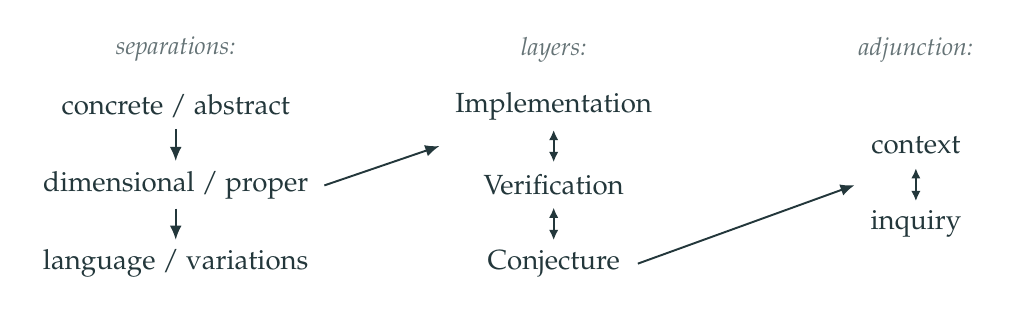
\begin{tikzpicture}[
      every node/.style={align=center, text=presentationgreen},
      layer/.style={minimum height=1.6em},
      columntitle/.style={font=\small\itshape, text=presentationgreen!70},
      arrow/.style={-{Latex[length=1.8mm, width=1.5mm]}, line width=0.7pt, presentationgreen},
      twoway/.style={{Latex[length=1.3mm, width=1.2mm]}-{Latex[length=1.3mm, width=1.2mm]}, line width=0.7pt, presentationgreen},
    ]
    \node[columntitle] at (-4.8, 0.72) {separations:};
    \node[columntitle] at (0, 0.72) {layers:};
    \node[columntitle] at (4.6, 0.72) {adjunction:};

    \node[layer] (implementation) at (0, 0) {Implementation};
    \node[layer] (verification) at (0, -1.0) {Verification};
    \node[layer] (conjecture) at (0, -2.0) {Conjecture};
    \draw[twoway] (implementation) -- coordinate (implementationtoverification) (verification);
    \draw[twoway] (verification) -- (conjecture);
    \node[fit=(implementation) (verification) (conjecture), inner sep=2pt] (layers) {};

    \node[layer] (concreteabstract) at (-4.8, 0) {concrete / abstract};
    \node[layer] (dimensionalproper) at (-4.8, -1.0) {dimensional / proper};
    \node[layer] (languagevariations) at (-4.8, -2.0) {language / variations};
    \draw[arrow] (concreteabstract) -- (dimensionalproper);
    \draw[arrow] (dimensionalproper) -- (languagevariations);
    \node[fit=(concreteabstract) (dimensionalproper) (languagevariations), inner sep=2pt] (separations) {};
    \draw[arrow] (separations.east) -- (layers.west |- implementationtoverification);

    \node[layer] (context) at (4.6, -0.5) {context};
    \node[layer] (inquiry) at (4.6, -1.5) {inquiry};
    \draw[twoway] (context) -- (inquiry);
    \node[fit=(context) (inquiry), inner sep=2pt] (poles) {};
    \draw[arrow] ([xshift=3pt]conjecture.east) -- (poles.west);
  \end{tikzpicture}%
}

% Process, first click: the conversations (C) form a graph T, joined by what passes
% between them (together); verification, the long bent arrow on the right, carries
% T to an exact replica G, the knowledge graph. Nodes, edges and letters take the
% colours of the marked words they stand for.
\newcommand{\processdiagram}{%
  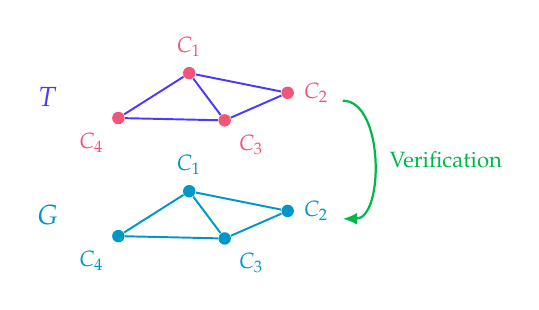
\begin{tikzpicture}[
      conversation/.style={circle, fill=conversationrose, inner sep=0pt, minimum size=4.5pt},
      concept/.style={circle, fill=graphblue, inner sep=0pt, minimum size=4.5pt},
      conversationname/.style={font=\footnotesize, text=conversationrose},
      conceptname/.style={font=\footnotesize, text=graphblue},
      message/.style={messageindigo, line width=0.7pt},
      link/.style={graphblue, line width=0.7pt},
    ]
    \node[conversation, label={[conversationname]above:$C_1$}] (t1) at (0, 0.6) {};
    \node[conversation, label={[conversationname]right:$C_2$}] (t2) at (1.25, 0.35) {};
    \node[conversation, label={[conversationname]below right:$C_3$}] (t3) at (0.45, 0) {};
    \node[conversation, label={[conversationname]below left:$C_4$}] (t4) at (-0.9, 0.03) {};
    \draw[message] (t1) -- (t4)  (t1) -- (t2)  (t1) -- (t3)  (t2) -- (t3)  (t4) -- (t3);
    \node[text=messageindigo] (togethergraph) at (-1.8, 0.3) {$T$};

    \begin{scope}[yshift=-1.5cm]
      \node[concept, label={[conceptname]above:$C_1$}] (g1) at (0, 0.6) {};
      \node[concept, label={[conceptname]right:$C_2$}] (g2) at (1.25, 0.35) {};
      \node[concept, label={[conceptname]below right:$C_3$}] (g3) at (0.45, 0) {};
      \node[concept, label={[conceptname]below left:$C_4$}] (g4) at (-0.9, 0.03) {};
      \draw[link] (g1) -- (g4)  (g1) -- (g2)  (g1) -- (g3)  (g2) -- (g3)  (g4) -- (g3);
      \node[text=graphblue] (knowledgegraph) at (-1.8, 0.3) {$G$};
    \end{scope}

    % Right of both graphs, clear of the C_2 labels: low looseness keeps the bend
    % long and narrow rather than round.
    \draw[-{Latex[length=1.8mm, width=1.5mm]}, verificationgreen, line width=0.8pt]
      (1.95, 0.25) to[out=0, in=0, looseness=0.9]
      node[right, xshift=2pt, font=\footnotesize, text=verificationgreen] {Verification}
      (1.95, -1.25);
  \end{tikzpicture}%
}


\begin{document}
\small
{\normalsize Hoapa, Helsinki Logic Group, 11 November 2026: slides and commentary (review copy)\par}
\slidehead{Opening (title slide)}{}
\begin{commentary}
\marked{Title}
\begin{itemize}
\item Hoapa = class of communication systems
\end{itemize}
- optimized for collective inquiry\par
- generalization seems relevant in Nature\par
\begin{itemize}
\item name: last slide
\end{itemize}
\marked{My name}
\begin{itemize}
\item unaffiliated, unspecialized
\item as good as their theories (football players-feet)
\item science \ensuremath{\cong} racing
\item School/univ dev of pilots \ensuremath{\cong} more and more demanding cars
\end{itemize}\vspace{2pt}
\begin{itemize}
\item I built my own car:
\end{itemize}
- by chance (brain soup)\par
- as an exercise/specs\par
\begin{itemize}
\item "what is… U\&B" \ensuremath{\to} I trusted it \ensuremath{\to} "took for a ride"
\end{itemize}\vspace{2pt}
\begin{itemize}
\item 1st step, labels: "the system doesn't know…"
\item last: "result stays in the abstract, as available resource, no movement back into the concrete"
\item vs. loss of knowledge, useless
\item complicated, non-trivial thing \ensuremath{\to} embryonic workshops
\end{itemize}\vspace{2pt}
\begin{itemize}
\item logic: odd workshops \ensuremath{\to} special workshops
\end{itemize}
\end{commentary}
\slidehead{Pitch}{1/40}
The core of my research consists in drawing inspiration from the philosophy of mathematics and the engineering of networks to formulate [a theory of work constrained by "\textcolor{permaculturegreen}{\emph{permacultural}}" logic: how to produce reusable results while preserving the conditions for future work]. Applied to collectives, it becomes an extension of the \textcolor{scienceblue}{\emph{scientific method}} which incorporates participatory democracy and sustainability.\par
\begin{itemize}
\item \textcolor{hoapaviolet}{\emph{[…]}}: one point of view among many
\item \textcolor{permaculturegreen}{\emph{Permacultural}}: abstracted into "concretely minimal, abstractly demanding"
\item \textcolor{scienceblue}{\emph{Scientific method}}: \newline well-regulated scientist–Nature relation + (ad hoc peer review \ensuremath{\hookrightarrow} universities \ensuremath{\hookrightarrow} economy)\newline \ensuremath{\to} \emph{well-regulated} network of relations among scientists, each retaining a well-regulated relation with Nature
\end{itemize}
\begin{center}\scalebox{0.62}{\pitchdiagram}\end{center}
\begin{commentary}
\marked{\textcolor{hoapaviolet}{[…]}}
\begin{itemize}
\item not a pitch but one of them
\item inherently perspectivist:
\item the world \ensuremath{\cong} a context \ensuremath{\cong} a system of points of view
\end{itemize}
\marked{\textcolor{permaculturegreen}{Permacultural}}
\begin{itemize}
\item abstraction of the agricultural technique
\end{itemize}\vspace{2pt}
\begin{itemize}
\item targets minimal imprint (your system \ensuremath{\cong} the natural's)
\item requires knowledge (your knowledge \ensuremath{\cong} the system's)
\end{itemize}
\marked{\textcolor{scienceblue}{Scientific}}
\begin{itemize}
\item an extension not a modification/relaxation
\end{itemize}\vspace{2pt}
\begin{itemize}
\item a protocol becomes an object of science
\item open, and scientists (anyone) expected to sign up for the most trustworthy
\end{itemize}\vspace{2pt}
\begin{itemize}
\item trust := whatt guarantees [ … ]
\item list obtained by "layers of complexity"
\end{itemize}
\marked{Inventory diagram}
\begin{itemize}
\item separations of concerns \ensuremath{\cong} specs
\item layers \ensuremath{\cong} levels of abstractions
\item poles of adjunction \ensuremath{\cong} motivation \& how-to
\end{itemize}
\end{commentary}
\slidehead{Sources}{2/40}
The authors it draws on are mathematicians (F.W. Lawvere, \textcolor{risingseateal}{\emph{A. Grothendieck}}), philosophers (C.S. Peirce, G. Simondon, G. Deleuze), and \textcolor{scienceblue}{\emph{scientists}} (S. Kauffman, J. Bowlby). In my project, these approaches meet in \textcolor{metaphysicsamber}{\emph{Albert Lautman}}’s philosophy of mathematics, as read by Fernando Zalamea (who has been supporting my work).\par
\begin{itemize}
\item \textcolor{risingseateal}{\emph{A. Grothendieck}}: gives a rich notion of creativity, the relative point of view, naturalness via the rising sea method, ecological thinking… the structure and destination of the project…
\item \textcolor{metaphysicsamber}{\emph{Albert Lautman}}: metaphysics as "problems the universe was going to run into no matter what", mathematics and physics as "effective theories answering those problems"…
\item \textcolor{scienceblue}{\emph{Scientists}}: because we're interested in each step of the evolution of the universe, from field theories to origins of life and attachment…
\end{itemize}
\transition{…Hoapa as an invariant in the effective theories we see}
\begin{commentary}
\marked{\textcolor{risingseateal}{A. Grothendieck}}
\begin{itemize}
\item workshops (embryonic)
\item \ensuremath{\cong} col. sci. method (specific use case)
\item \ensuremath{\cong} recursive elem. in G-evol (in Nature)
\end{itemize}
\marked{\textcolor{metaphysicsamber}{Albert Lautman}}
\begin{itemize}
\item bio (1930, anticipator, non-reductionist)
\item more recent anchor
\end{itemize}\vspace{2pt}
\begin{itemize}
\item demystifying metaphysics
\item movement from metaphysics to effective theories
\item giving a context to mathematics, physics… Hoapa
\end{itemize}
\marked{\textcolor{scienceblue}{Scientists}}
\begin{itemize}
\item each step = a correspondance test
\end{itemize}
\end{commentary}
\slidehead{Thesis}{3/40}
My main thesis states that in a system that puts the dialectic between concrete and abstract to \textcolor{energyorange}{\emph{work}} (brain, computer, community), the relation between concrete substrate and logical labor must be a resource entirely \textcolor{dedicationmagenta}{\emph{dedicated}} to the design and application of representations and algorithms. A form of separation between two kinds of \textcolor{decompositionocean}{\emph{decomposition}}—analytic (as in prime factorization) and synthetic (as in vector coordinates relative to a basis)—is a guiding principle, informed by Lautman, which can keep this relation fruitful: in a community, between thinkers and the knowledge they produce.\par
\begin{itemize}
\item \textcolor{energyorange}{\emph{Work}}: explosion vs. engine, the role of constraints;\newline engine vs. organism, the role of closure;\newline engine vs. computer, the role of the "abstract loop"\newline (Stuart Kauffman, "Beyond Physics" talk)
\item \textcolor{dedicationmagenta}{\emph{Dedicated}}: as in computers, in cells, in brains, in communities
\item \textcolor{decompositionocean}{\emph{Decomposition (Lautmanian)}}: synthetic (dimensional) \ensuremath{\longleftrightarrow} analytic (proper)
\end{itemize}
\begin{commentary}
\marked{\textcolor{energyorange}{Work}}
\begin{itemize}
\item engine \ensuremath{\to} Peter Atkins (extending physics)
\end{itemize}
- work = "constrained release of energy into a few degrees of freedom"\par
\begin{itemize}
\item organism \ensuremath{\to} Kauffman (origins of life)
\end{itemize}
- closures = "collective work which constructs and maintains the constraints that enable those processes" (constraint, work-task, catalytic)\par
\begin{itemize}
\item computer (also brain, genome, communities) \ensuremath{\to} Pattee (symbolic and dynamical)
\end{itemize}
- "physical activity is recorded in symbols, which can be stored, manipulated and interpreted to guide further physical activity" (von Neumann, Peirce)\par
\begin{itemize}
\item logic: formal system and realization (Lautman and others, for us: abstract/concrete)
\item Hoapa = a system of constraints, open but capable of closure, and optimized for symbolic work
\end{itemize}
\marked{\textcolor{dedicationmagenta}{Dedicated}}
\begin{itemize}
\item evident in computers \& genome:
\item the hardware is dedicated to running the software
\end{itemize}\vspace{2pt}
\begin{itemize}
\item brains are less clear-cut:
\item internal concrete/abstract divides, as in math and code (multilevel vs. one level)
\end{itemize}\vspace{2pt}
\begin{itemize}
\item communities are "degenerate":
\item concrete substrate (lives) coupled, dependent on the abstract (science \ensuremath{\to} economy)
\item Hoapa: clear distinction between "living your life" and "participating in specific collective work, including inquiry"
\end{itemize}
\marked{\textcolor{decompositionocean}{Decomposition}}
\begin{itemize}
\item If we think of a space being decomposed:
\item dim = decompose through the structure of the ambient space
\item prop = decompose through the structure of the element itself
\end{itemize}\vspace{2pt}
\begin{itemize}
\item at the community level \ensuremath{\to} knowledge
\item brains are like vectors \ensuremath{\to} very complex Venn diagram with lots of overlapping world-maps/brains
\item documented statements like prime factorization \ensuremath{\to} a list
\item Hoapa: "system that uses these decompositions to implement the dedicated relation between concrete and abstract"
\end{itemize}
\end{commentary}
\slidehead{Theory of work}{4/40}
The physical starting point is that work depends on \textcolor{constraintred}{\emph{constraints}} that channel energy into particular effects. In living systems, activity also helps \textcolor{permaculturegreen}{\emph{maintain}} the machinery that makes further activity possible. \textcolor{abstractmirrorblue}{\emph{Abstract}} representations and algorithms enable a system to retain and share experience, discover relations, construct and test possibilities, revise its own means of understanding and action, and turn results into conditions for further work. This makes the relation between concrete conditions and abstract operations a powerful resource. Lautman supplies a way to investigate such relations through the mathematical and physical constructions that give them substance; Peirce, Simondon, and Kauffman help connect the question to living beings, their environments, and their practices of understanding. Hoapa's proposed separation between thinkers and the organization of knowledge is an engineering approach to developing this potential.\par
\begin{itemize}
\item \textcolor{constraintred}{\emph{Constraints}}: effects — Maintain : closure — Abstract : secondary loop
\end{itemize}
\begin{commentary}
\begin{itemize}
\item "Constraints give you effects, closure gives you continuity, the abstract gives you extra possibilities"
\end{itemize}
\end{commentary}
\slidehead{Process}{5/40}
Hoapa is designed as a network of small \textcolor{conversationrose}{\emph{conversations}} in which one group's work becomes another group's starting point. A question brings participants \textcolor{messageindigo}{\emph{together}}; their discussion produces a document that others can examine, challenge, or develop. These documents form a growing map of questions, concepts, arguments, and dependencies: a knowledge \textcolor{graphblue}{\emph{graph}}. So that contributions can differ and come unforced, the system gives participants control and equal standing (they all play by the same rules they themselves manage). Knowledge acquires structure \textcolor{independencecopper}{\emph{independently}} of the structure of its producers, be it social, political, economic…\par
\begin{itemize}
\item \textcolor{conversationrose}{\emph{Conversation}}: modeled after citizen assemblies (helps autonomy, role-symmetry, modularity… control and equal standing)
\item \textcolor{messageindigo}{\emph{Together (concurrency)}}: message passing style, as in the actor model or \ensuremath{\pi}-calculus
\item \textcolor{graphblue}{\emph{Graph}}: typed knowledge graphs, which are versioned, multiplex, homotopical, federated…
\item \textcolor{independencecopper}{\emph{Independently}}: respecting the concrete/abstract separation of concerns and dedicated relation between the two
\end{itemize}
\begin{center}\scalebox{0.8}{\processdiagram}\end{center}
\begin{commentary}
\marked{Overview diagram}
\begin{itemize}
\item convs \ensuremath{\to} atoms of reflexion
\item concurrency \ensuremath{\to} network of reflexion
\item graphs \ensuremath{\to} structured memory of reflexion
\end{itemize}
\marked{\textcolor{conversationrose}{Conversation}}
\begin{itemize}
\item amazing results when experimented in politics
\end{itemize}\vspace{2pt}
\begin{itemize}
\item random selection and consensus \ensuremath{\leftrightarrow} "play by the same rules"
\item "let it crash" in Erlang
\end{itemize}
\marked{\textcolor{messageindigo}{Together}}
\begin{itemize}
\item these concurrency models follow Lautman decomposition:
\end{itemize}
- actors are "synthetic" agents\par
- their messages "analytic" decomposition\par
\marked{\textcolor{graphblue}{Graph}}
\begin{itemize}
\item the free "base" layer = verbatim record of "spontaneous" back and forth
\item refinement into specialized/pruned graphs (UTL)
\end{itemize}\vspace{2pt}
\begin{itemize}
\item recap, ideas: conv (maelstrom \ensuremath{\to} born) \ensuremath{\to} concurrency (medium \ensuremath{\to} travel) \ensuremath{\to} graph (structure \ensuremath{\to} land)
\end{itemize}
\marked{\textcolor{independencecopper}{Independently}}
\begin{itemize}
\item not much change in content (broader scope)
\item impact is on diffusion \& accessibility, trust, usage \& usefulness, representativity, control of new technologies…
\end{itemize}
\end{commentary}
\slidehead{Partial diagram}{6/40}
\begin{center}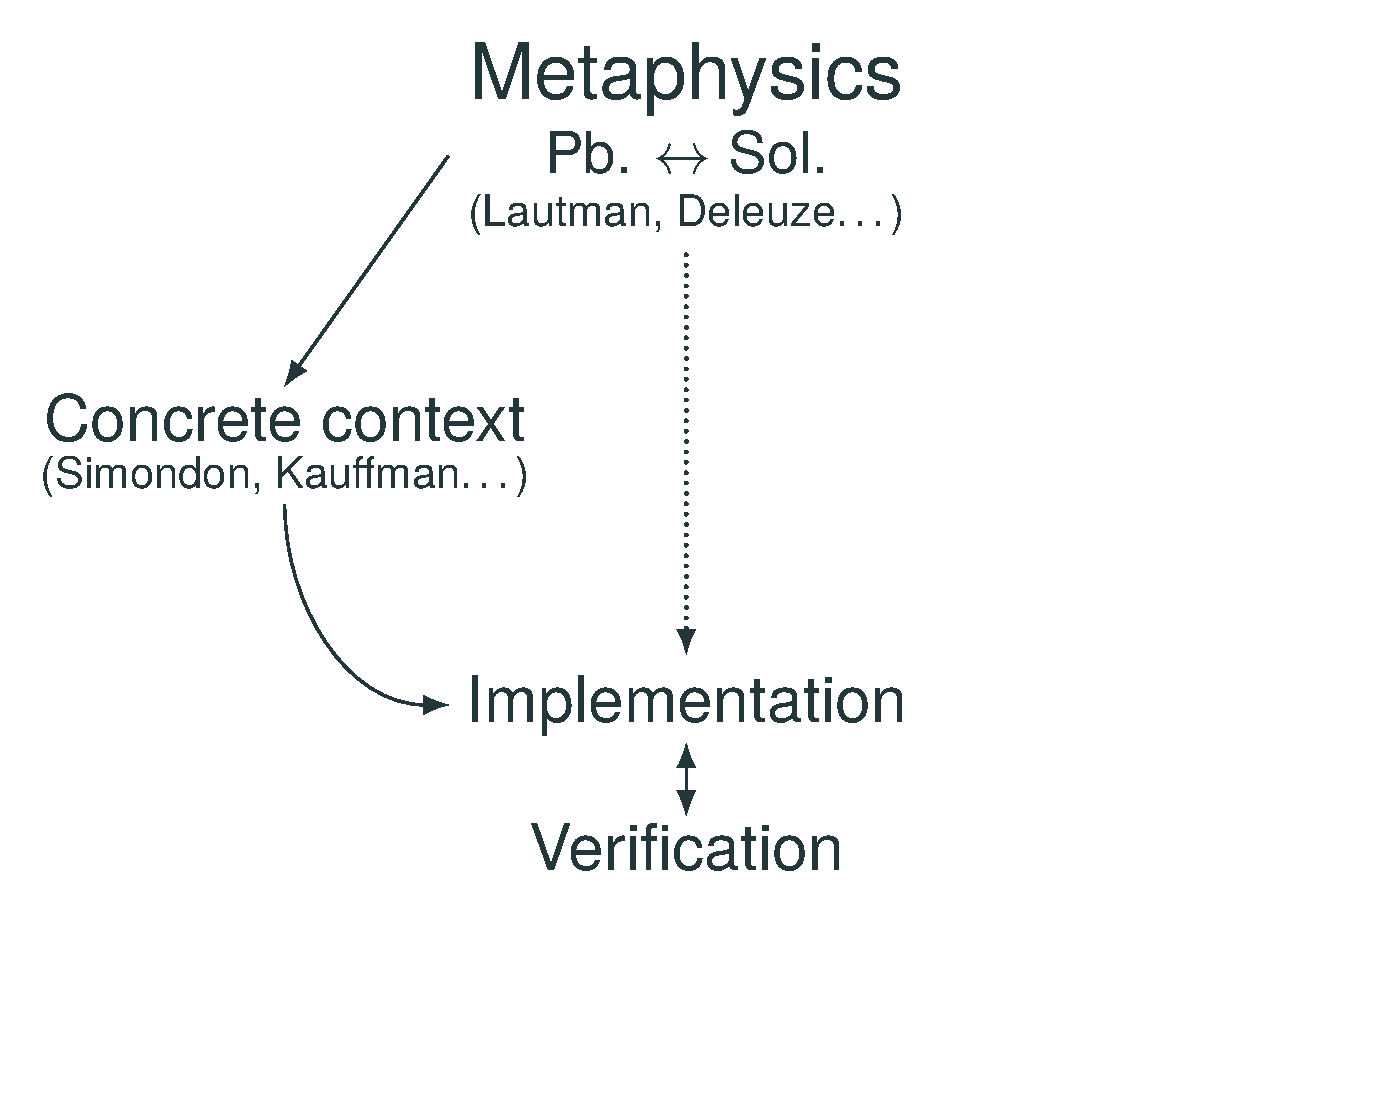
\includegraphics[width=0.38\linewidth]{talk_hlg_111126_diagram_partial.pdf}\end{center}
\begin{commentary}
\begin{itemize}
\item Lautman's demystified metaphysics
\item \ensuremath{\to} theory of abstract work
\item \ensuremath{\to} implementation, verification, conjecture
\end{itemize}
\end{commentary}
\slidehead{Verification}{7/40}
The communication protocols specify how these conversations proceed and how their results enter the shared documentation. Software is used as a \textcolor{refereeyellow}{\emph{referee}} and is itself subject to modification by the conversations. Alongside the conversation process, a mathematical \textcolor{verificationgreen}{\emph{verification}} layer is being developed in cubical Agda, a language in which proofs can be checked by a computer. One existing result establishes that consistently renaming \textcolor{participantsplum}{\emph{participants}} cannot change the checker's verdict. The broader aim is to make the system's promises precise enough to test and prove.\par
\begin{itemize}
\item \textcolor{refereeyellow}{\emph{Referee}}: or automation as \_liberation from control mechanisms\_, from the necessity to have management
\item \textcolor{verificationgreen}{\emph{Verification}}: machine-checks that the record of each conversation is well-formed according to the protocol, never that its conclusions are true
\item \textcolor{participantsplum}{\emph{Participants}}: the protocol is blind to identity of contributors, which means it can't count on specialization (…is knowledge lost?)
\end{itemize}
\slidehead{Conjecture}{8/40}
The project seeks a mathematical correspondence—an \textcolor{adjunctioncrimson}{\emph{adjunction}}—between two poles. One organizes inquiry through conversations, verification, and knowledge graphs. The other represents mathematical contexts and the different perspectives through which they can be investigated. The conjecture is guided by an intuition prompted by the perspectival nature of the world: our different understandings of it invite discussion, without presuppositions, from which something the world can reuse may \textcolor{emergencecoral}{\emph{emerge}}. The conjecture asks whether a \textcolor{universalpropertyblue}{\emph{universal property}} can distinguish Hoapa’s organization from alternatives. This talk will explore a candidate in which methods are represented by logics and mathematical worlds by the inner models they generate.\par
\begin{itemize}
\item \textcolor{adjunctioncrimson}{\emph{Adjunction}}: context \& inquiry,  perspectivism \& praxis, structure \& genesis/recursion…
\item \textcolor{emergencecoral}{\emph{Emerge}}: points to the recursive nature of evolution: physics to biology, biology to psychology…
\item \textcolor{universalpropertyblue}{\emph{Universal property}}: "specialness" in mathematics \ensuremath{\to} optimality in engineering
\end{itemize}
\begin{commentary}
\marked{\textcolor{adjunctioncrimson}{Adjunction}}
\begin{itemize}
\item see later
\end{itemize}
\marked{\textcolor{emergencecoral}{Emerge}}
\begin{itemize}
\item "Heavy machinery" found in Simondon's view: how beings come to be? context of potentials, coevolution, never exhausting it
\item new candidates for individuation come from new context (AGI)
\end{itemize}\vspace{2pt}
\begin{itemize}
\item reusability: \emph{return} to context or "standalone byproduct": new context, \emph{replay} (see later)
\end{itemize}
\marked{\textcolor{universalpropertyblue}{Universal property}}
\begin{itemize}
\item a translation
\end{itemize}
\end{commentary}
\slidehead{Rising sea as a reason to believe in permacultural logic}{9/40}
Video: P. Deligne, \emph{L'œuvre d'Alexandre Grothendieck} (Nice, 1996), the first 1'12, with English subtitles (deligne\_rising\_sea.mp4). Click to play.\par
\begin{center}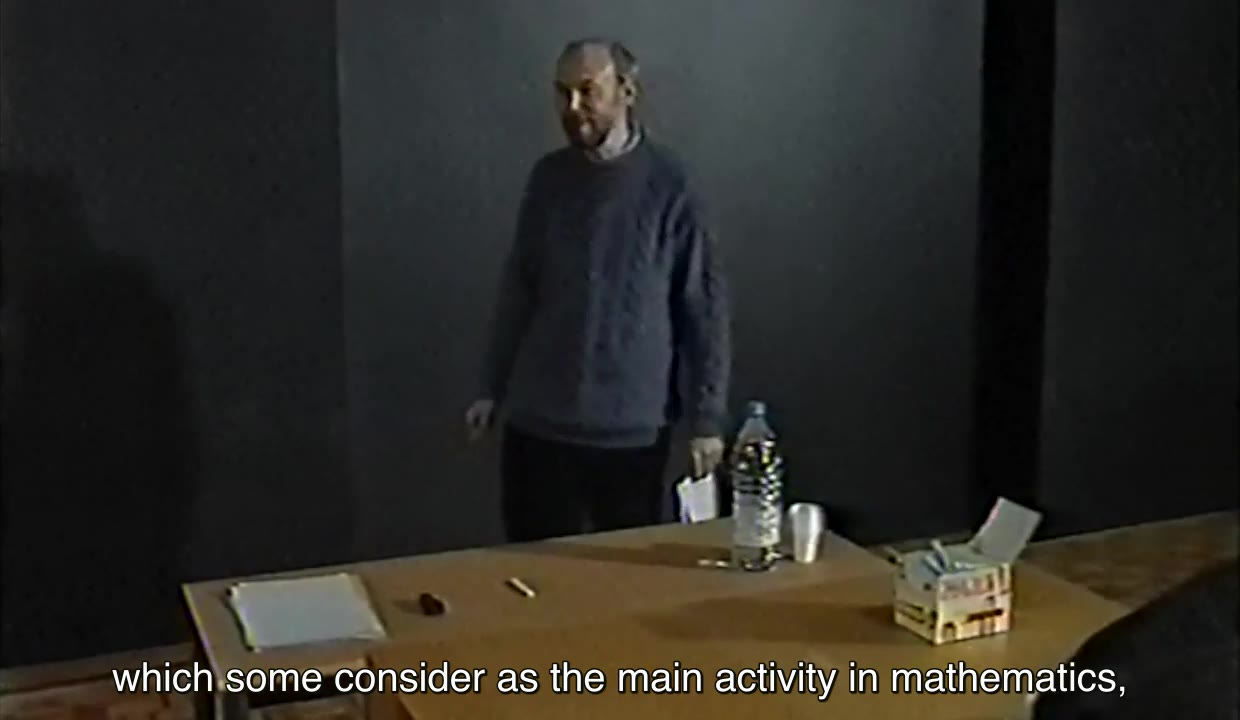
\includegraphics[width=0.3\linewidth]{deligne_rising_sea_poster.jpg}\\{\footnotesize\color{gray}Video: P.~Deligne, \emph{L'œuvre d'Alexandre Grothendieck}, Nice, 1996 (first 1'12)}\end{center}
\begin{commentary}
\begin{itemize}
\item Permacultural logic is an outgrowth of my work on Hoapa, not one of its constituents
\item It could be that Hoapa's optimality is true and the permacultural interpretation of logic is false
\item main reason to believe is not technical, but that the rising sea methodology works
\end{itemize}
\end{commentary}
\slidehead{Permacultural logic}{10/40}
The project also looks for this pattern inside logic, where "permaculture" is understood broadly as the two-step process of (1) getting to know one's context as much as possible, (2) acting minimally in a manner that will enhance one's condition while preserving and enriching the context. A proof may begin with a provisional assumption (borrow), derive a conclusion (work), and turn the derivation into a conditional statement that later proofs can use (return) or start afresh from (\textcolor{replayolive}{\emph{replay}}). Hoapa investigates this borrow–work–replay pattern as a possible logical expression of its permacultural ambition: the \textcolor{harmonyorchid}{\emph{harmony}} between receiving and giving back.\par
\begin{itemize}
\item \textcolor{harmonyorchid}{\emph{Harmony}}: as in Gentzen, type theory, Hilbert's axiomatic method
\item \textcolor{replayolive}{\emph{Replay}}: the hidden part of logic that makes logic work
\end{itemize}
\begin{commentary}
\marked{\textcolor{harmonyorchid}{Harmony}}
\begin{itemize}
\item Gentzen in intro/elim
\item in type theory with how to construct a type and how to use a type
\item Hilbert in axioms and metamathematical theory (in the vision of Lautman)
\end{itemize}\vspace{2pt}
\begin{itemize}
\item My eureka moment came from a biological analogy: "A cell draws on a proton gradient to produce ATP for new work, while consuming fuel to replenish the gradient, some of that work maintains the machinery that keeps the cycle going"
\item see later
\end{itemize}
\marked{\textcolor{replayolive}{Replay}}
\begin{itemize}
\item return: novelty \ensuremath{\to} into the context, replay: novelty \ensuremath{\to} into a new process
\end{itemize}\vspace{2pt}
\begin{itemize}
\item As an intuition:
\item visible part is the feedforward: math goes from problems to results and from results to problems
\item hypothesis: "you can't see the feedback, but for the structural rules to hold (\ensuremath{\cong} "the system to be sustainable"), there must be a form of non-exhaustion (Simondon) and positive feedback (cybernetics)"
\end{itemize}
\end{commentary}
\slidehead{Development}{11/40}
The architecture of a "mature" Hoapa system is both demanding—to respect its constraints—and—by virtue of presuppositionlessness—\textcolor{unpredictablecyan}{\emph{unpredictable}}. Autonomous open-science workshops could make these ideas tangible and seed larger systems, embracing both pragmaticism and experimentalism. Their first requirement is usefulness: knowledge sharing must be truly at \textcolor{stakebrown}{\emph{stake}}, so that the organization develops through serving a real purpose. Concretely, I envision something based on the philosophy of "document-driven-development", where \textcolor{documentationink}{\emph{documentation}} gradually replaces the instructor, both as the joint source of truth and the manager of the process.\par
\begin{itemize}
\item \textcolor{unpredictablecyan}{\emph{Unpredictable}}: collective inquiry helps determine how collective inquiry is organized
\item \textcolor{stakebrown}{\emph{Stake}}: what distinguishes and makes citizen assemblies efficient; you can't simulate life or understanding
\item \textcolor{documentationink}{\emph{Documentation}}: does in the Lautmanian-analytic what specialization does in the synthetic agents: shared source and management, but "softer"
\end{itemize}
\begin{commentary}
\marked{\textcolor{unpredictablecyan}{Unpredictable}}
\begin{itemize}
\item "only collective intelligence should shape what collective intelligence should be"
\item the same form of non-ergodicity as biology
\end{itemize}
\marked{\textcolor{stakebrown}{Stake}}
\begin{itemize}
\item stakes are facilitators of consensus (in citizen assemblies, high gain)
\item In Hoapa, so are role-symmetry and general equalitarian conditions, openness, anonymity… (low cost)
\end{itemize}
\marked{\textcolor{documentationink}{Documentation}}
\begin{itemize}
\item Think "operational/executable documentation", see later
\end{itemize}
\end{commentary}
\slidehead{A park}{12/40}
Hoapa can also operate at small scales and with only the "base layer of complexity" which separates the role-symmetric agents from the typed documentation they produce.\par
For instance we could have a neighborhood "manage" its local park via a protocol in which the motivated residents discuss how it could be enhanced, and produce a to-do list for its maintenance.\par
Here it is crucial to understand that the system can preserve its advantageous mathematical, social and engineering properties if it is \textbf{only} a communication system, and not a full management system which also enacts in reality what has been discussed in the abstract.\par
Its task is to chart the world and design appropriate algorithms, not interfere with and certainly not control it. (That would kill all the carefully crafted separations of concerns, starting with the role-symmetry of agents, because it necessarily introduces some hierarchical structure and tension—for basically the same reasons you can share an idea with the entire world without losing it, but you can't do that with a loaf of bread.)\par
Hoapa protocols can interact with the world only behind buffers which respect individual freedom:\par
\begin{itemize}
\item If it needs something it simply asks for it, and expects those needs to be met (for instance, if it uses the internet, it states via a self-reflective conversation how much bandwidth it needs, and specifies the characteristics of its network). Individuals or communities, outside of the protocol, would then respond to those needs without compensation.
\item If it wants something to be known it simply makes it as available and accessible as possible, which includes a pedagogical effort in presentation and terminology. But it can't advertise, at the risk of favoring certain targets over others.
\end{itemize}
In either direction, we can think of Hoapa as a coach in sports: its domain of action is preparation and strategy, but it can never enter the field of play or control the players. The game belongs to the players.\par
In this example, we can imagine an institution/Hoapa hybrid in which the city government has delegated the supervision of the park to the protocol, but it's still the paid workforce of gardeners which will perform the tasks suggested by the protocol. But ideally, in the spirit of the protocol, it would be only voluntary work, suggested by the protocol but decided at the level of the individuals and communities.\par
\transition{Which makes Hoapa protocols especially well suited to organize the open source economy.}
\slidehead{Open source}{16/40}
Because open source produces code, it mostly "lives in the abstract". Historically, it has also used a lot of voluntary labor. So it is by design a process that respects the separation of concerns Hoapa systems start with.\par
The main recurring problem open source projects face is scalability and continuation beyond the circle of core contributors and maintainers, usually the instigators of the project: because open source projects are structured around "circles of knowledge and influence", which is in essence a hierarchy, it is very likely to terminate the moment the inner circle quits.\par
Hoapa revokes the privileges of the inner circle, distributes the workload evenly and transfers all the essential knowledge from the original designer's minds into a strictly typed and \textcolor{documentationink}{\emph{operational documentation}}.\par
While this is more demanding in the early stages of the process, it pays off by making the project truly scalable and persistent (not persistent in the sense of a capitalistic endeavor, which always needs to grow and colonize new markets, but closer to how ecosystems work, with minimalism and circularity).\par
\transition{The same arguments can be used to suggest a reform of how science is conducted.}
\begin{itemize}
\item \textcolor{documentationink}{\emph{Operational documentation}}: using team semantics and provenance, what must remain traceable for others to understand, revise, and continue the work (as an extension to the collective of Knuth's literate programming)
\end{itemize}
\begin{commentary}
\marked{\textcolor{documentationink}{Operational documentation}}
\begin{itemize}
\item \emph{literate programming} as working model (the great missed opportunity of software development)
\item better model is team semantics and provenance
\item "for the work to have document-to-document continuity, as opposed to brain-to-brain or self-to-self, the documentation needs to show how a result was obtained, what it depends on, and what may need reconsidering when those dependencies change, etc."
\end{itemize}
\end{commentary}
\slidehead{Science}{18/40}
\sout{Universities organize inquiry through hierarchies that also distribute funding, employment, and recognition. These dependencies influence which questions can be pursued and whose contributions are heard.}\par
Universities are extremely hierarchical political machines whose ties to reality are clearly not behind buffers, which impair their capacity to describe the world they inhabit.*\par
While the scientific method, in the domains where it is applicable, makes claims answerable to evidence and correction, it doesn't prevent other types of evils. Notably a mismanagement of efforts toward certain technologies at the expense of understanding, the fragmentation of the study of Nature into opposing departments, the proliferation of opaque jargons, the insistence that there exists a "view from nowhere", the enclosure of knowledge behind paywalls, proprietary tools, and restricted access, the depreciation of errors and failures, etc.\par
Hoapa protocols, on the other hand, are ideal for the realization of what citizen science promised to be, but only marginally developed. In a real and, hopefully, demonstrable sense, they are an extension of the Galilean scientific method to the collective.\par
In the Hoapa extension, we define how scientists are supposed to converse among themselves, and how they should refine and store information into a strictly typed and operational technical \textcolor{languageamethyst}{\emph{language}}. Our conjecture is that a universal property can distinguish Hoapa among organizations pursuing this work.\par
Hoapa protocols are designed for education, as part of their mandate to treat everybody on an equal footing. What is removed with the status is not the knowledge, but the hunt for the status, and at the same time it resituates the obligation to make one's specialized knowledge accessible to others.\par
Crucially, each individual practitioner gets to decide what questions are worth pursuing, opening a path to restoring science’s sense of purpose from the ground up.\par
\transition{And the organization of inquiry is itself something we can try to understand mathematically.}
\begin{itemize}
\item \textcolor{languageamethyst}{\emph{Language}}: "Learn once, write everywhere" \ensuremath{\leftarrow} a shared conceptual landscape built through explicit and systematic comparisons (interpretation, equivalence, coherence…)
\end{itemize}
\begin{commentary}
\marked{*}
\begin{itemize}
\item "And all science, when we do not understand it as an instrument for power and domination, but as an adventure in knowledge undertaken by our species through the ages, is but this harmony, more or less wide and more or less rich from one period to the other, which unfolds over the generations and centuries, by the gentle counterpoint of all the themes emerging in turns, as if summoned from the abyss, to join and embrace in her" (Grothendieck, R\&S)
\item "From a semiotical and philosophical perspective, the general method is fascinating: to understand something, consider all possible points of view and search for a structural connection between them. Only then you will be approaching true knowledge. A systematic use of the liberty and multiplicity of topos theory in our ordinary life would have huge consequences on tolerance, ethics, politics, and social action: an example of how high mathematical practice would transform our everyday practice." (Zalamea, 'Grothendieck’s 40 Main Years: A Unitary Vision Through the TSK Models')
\end{itemize}
\marked{\textcolor{languageamethyst}{Language}}
\begin{itemize}
\item From React's slogan: systematize correspondences in the vocabulary and symbols across specialized domains
\item Example: know berry picking and read about electronics, find a technical word you know and know you can trust your knowledge of it
\end{itemize}\vspace{2pt}
\begin{itemize}
\item How? homotopy theoretic work on the Hoapa graphs
\item third separation: 1. concrete/abstract 2. synthetic agents/analytic documentation 3. language/variations
\end{itemize}\vspace{2pt}
\begin{itemize}
\item technical bridge: "Awodey and Forssell’s First-Order Logical Duality, which explicitly connects with the Grothendieckian setting, relating categories presenting theories to topological groupoids of models and their isomorphisms, using topos theory to establish a syntax–semantics duality."
\end{itemize}
Explicit example: a berry patch and a charging capacitor\par
\begin{itemize}
\item If you pick at random, the berries you find are proportional to the berries left. So your basket fills fast at first, then slower and slower: picked = all \ensuremath{\times} (1 - e\textasciicircum{}(-t/\ensuremath{\tau})).
\item A capacitor charging through a resistor follows exactly the same curve: V = V\ensuremath{_0} \ensuremath{\times} (1 - e\textasciicircum{}(-t/\ensuremath{\tau})), with \ensuremath{\tau} = RC.
\item These aren't just alike: both are the same equation, dx/dt = (target - x)/\ensuremath{\tau}.
\end{itemize}
\end{commentary}
\slidehead{Mathematics}{21/40}
All of the above applies in mathematics as well, but here the connection goes \textcolor{emergencecoral}{\emph{further}}: mathematics also supplies the language in which the organization of mathematical work can itself be investigated. Hoapa’s formalization uses Cubical Agda, bringing together homotopy type theory, computer-checked proofs, and a line of thought connecting Alexander Grothendieck’s ideas about homotopy types and higher groupoids with Vladimir Voevodsky’s univalent foundations.\par
Hoapa proposes to carry this connection into the organization of collective inquiry itself. This ambition echoes Grothendieck’s memoirs, which weave together reflections on creativity, mathematical practice and mathematics itself.\par
\transition{Grothendieck also questioned the ecological consequences of scientific activity; Hoapa approaches that concern by asking how understanding a world can help us inhabit it.}
\begin{itemize}
\item \textcolor{emergencecoral}{\emph{Further}}: a method of articulating a context can generate a new context for further inquiry (in math and logic, in generalized evolution)
\end{itemize}
\begin{commentary}
\marked{\textcolor{emergencecoral}{Further}}
\begin{itemize}
\item As before: the means developed to understand a context \ensuremath{\to} new context for further inquiry (Lautman: structure \ensuremath{\to} genesis)
\item Sources: Kennedy, Magidor and Väänänen - "Inner Models from Extended Logics", or Kennedy's essay "On the “Logic without Borders” Point of View" as concrete examples of what “a mathematical world generated through specified expressive resources” can mean
\end{itemize}
\end{commentary}
\slidehead{Generalized permaculture}{22/40}
I believe Hoapa protocols can stage and target the kind of recursive and self-reflective patterns just mentioned, in the ecosystem, by generalizing the concept of permaculture and applying it to a vast majority of human endeavors. Permaculture could in effect become the default mode of being of humanity, following this very simple algorithm:\par
\begin{itemize}
\item Make a very detailed and executable map of your environment, including your imprint on it.
\item Use it to figure out what is best for both you and your environment, and do it (which becomes the default if individual freedom replaces "investability" as the condition for action).
\end{itemize}
This is where the "layers of complexity" which respect and target perspectivism, decentralization, autonomy, openness to peers, expressiveness, transparency, scalability and self-reflection, start to be really useful.\par
\transition{To tend a place is also to attend to the relations that sustain it—and those relations lead us into a network.}
\begin{commentary}
\begin{itemize}
\item Not permacultural logic: what Nature may be doing
\item Generalized permaculture: what we should be doing
\end{itemize}
\end{commentary}
\slidehead{Networks}{24/40}
In all the preceding examples we've looked at instances of Hoapa protocols in isolation, but each of them would be better envisioned as a node of a vast network.\par
A mature protocol regulating a park would necessarily have typed conversations with other park protocols, especially those close by, to share information and reuse each other's research. It would also have ties to all the independent but interlinked networks a city would be made up of: electricity grid, water management, transportation, agriculture… and then beyond the city limits, into all sorts of other communities organized through protocols, each bringing its own point of view, from playground design to natural philosophy.\par
A park’s investigation of soil and water becomes useful to another park; a software improvement made for its documentation becomes available to other projects; a scientific question raised locally finds research communities elsewhere equipped to pursue it. The park community’s teaching material can help newcomers elsewhere. And communities can help one another translate documentation, test proposals, or investigate disagreements. Records of failed attempts can spare others the same mistakes.\par
In all of this, each protocol is both an agent and a recipient of \textcolor{careterracotta}{\emph{care}}, as a concrete ecosystem as well as an abstract community of participants.\par
\begin{itemize}
\item \textcolor{careterracotta}{\emph{Care}}: Hoapa’s generalization of attachment theory (biology, psychology) into a two-step cyclic algorithm\newline 1. In a given network, the evolution toward maturity of newer elements is taken care of by the\newline mature elements already present in the network\newline 2. In turn, those newer elements become mature and take care of a new generation of elements
\end{itemize}
\begin{commentary}
\marked{\textcolor{careterracotta}{Care}}
\begin{itemize}
\item attachment theory as effective theory which we can relate to metaphysical dialtectics/problems , with "traces of Hoapa"
\item A whole other avenue of research, another "layer of complexity" to try and locate in natural systems
\end{itemize}\vspace{2pt}
\begin{itemize}
\item Some related structures:
\item Lautman's "solidarity networks"
\item Yoneda lemma
\end{itemize}\vspace{2pt}
\begin{itemize}
\item game-theoretic semantics, particularly the tradition of Hintikka, Sandu, and Väänänen. For instance 'Abramsky and Väänänen - From IF to BI: A Tale of Dependence and Separation' ("In game semantics, negation exchanges the verifier’s and falsifier’s roles: a mathematical precedent for treating reciprocity of roles as part of an interaction’s structure")
\end{itemize}
\end{commentary}
\slidehead{Informal recap diagram}{26/40}
\begin{center}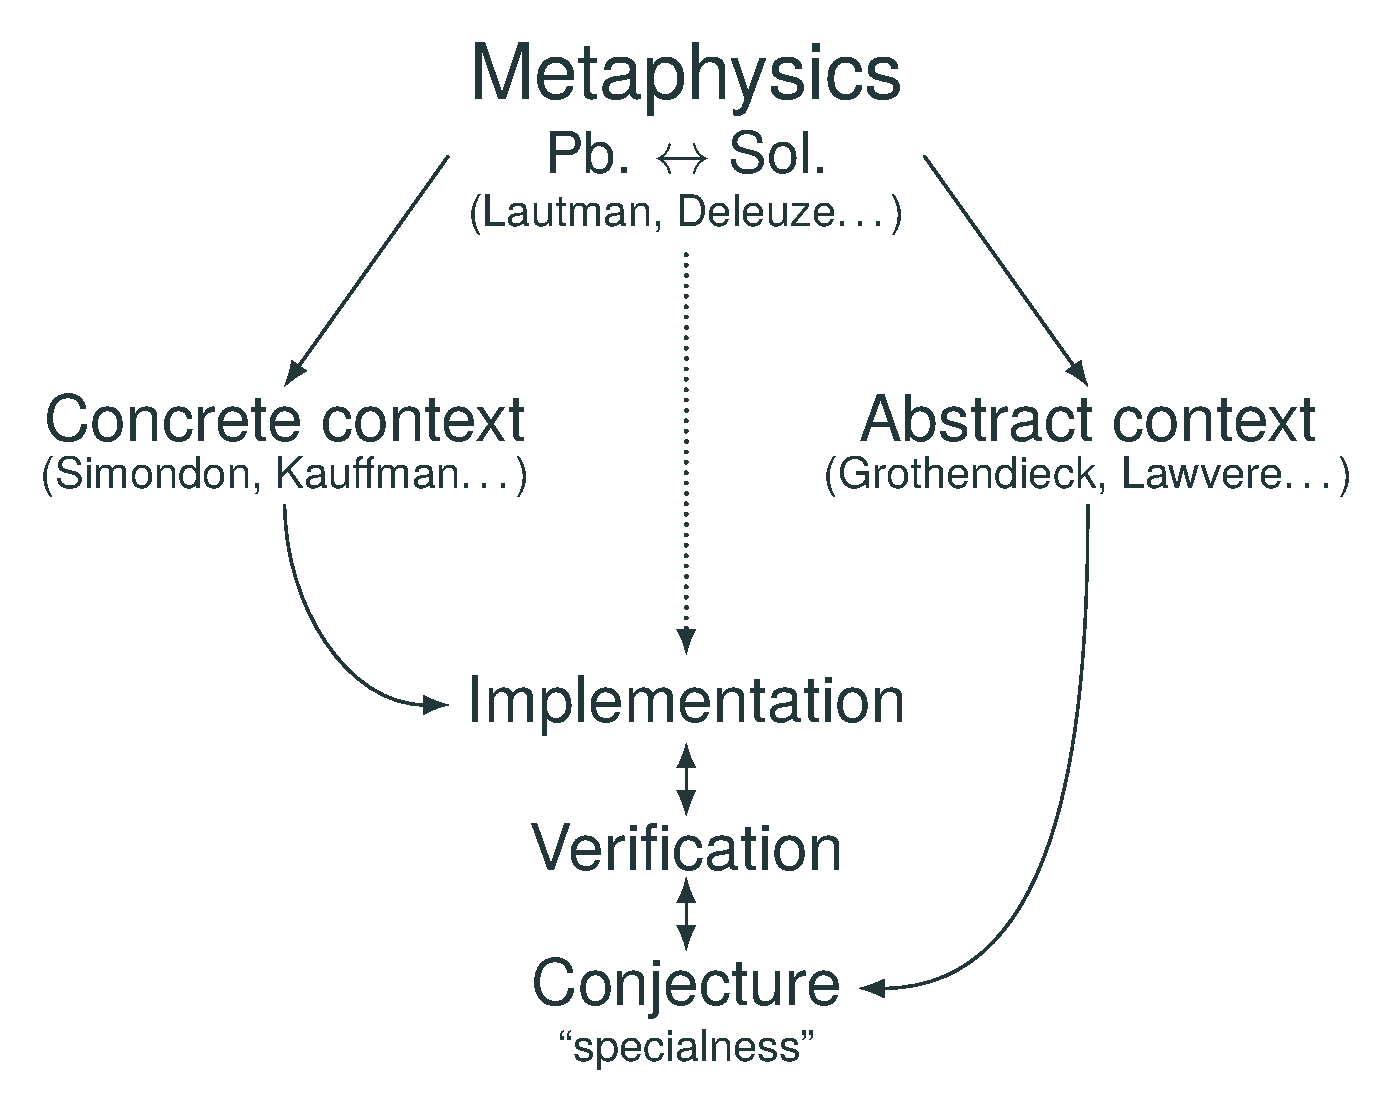
\includegraphics[width=0.38\linewidth]{talk_hlg_111126_diagram_full.pdf}\end{center}
\begin{commentary}
\begin{itemize}
\item looking for a mathematical setting in which the questions motivating the design become questions we can investigate precisely
\end{itemize}
\end{commentary}
\slidehead{Motivations and goals}{27/40}
To motivate its adoption and distinguish Hoapa from other “interesting projects” we can attach buzzwords to, I need a mathematical reason for organizing inquiry this way. The goal is to characterize Hoapa by a universal property, in a setting that represents both the contexts it investigates and alternative ways of investigating them.\par
If the conjecture succeeds, this universal property would translate into a claim of \textcolor{optimalitygold}{\emph{optimality}} for any implementation satisfying its conditions. The world we inhabit must explain why those conditions matter. Hoapa is also its own experiment: implementing its protocols lets us test the conjecture's claims.\par
\textcolor{hoapaviolet}{\emph{Perspectivism}} motivates this ambition; \textcolor{presuppositionlessnessteal}{\emph{presuppositionlessness}} guides the response. The world has already produced different beings, experiences, skills, and ways of understanding. Their contributions must be able to enter the inquiry without their worth being decided in advance by a hierarchy or an established division of knowledge. What the world has already developed becomes material for collective work; what that work will produce remains open.\par
\begin{itemize}
\item \textcolor{optimalitygold}{\emph{Optimality}}: the constraints imposed on a process, in a given context, to achieve an intended outcome\newline constraints = the protocol ; process = collective inquiry ; context = this world ; outcome = understanding that enables generalized permaculture to be enacted
\item \textcolor{hoapaviolet}{\emph{Perspectivism}}: global understanding is assembled from local views, with obstructions to their integration retained as information
\item \textcolor{presuppositionlessnessteal}{\emph{Presuppositionlessness}}: applied to protocols, a principle saying we need common rules, open rules with equally distributed power to revise them, and only the rules needed to make communication possible
\end{itemize}
\begin{commentary}
\marked{\textcolor{optimalitygold}{Optimality}}
\begin{itemize}
\item \emph{understanding} = demanding abstract work
\end{itemize}
\marked{\textcolor{hoapaviolet}{Perspectivism}}
\begin{itemize}
\item Lautman anticipates sheaf-theory with global/local
\item Philosophical perspectivism with its long tradition (Deleuze, Spinoza)
\item in HLG scope: Ehrenfeucht–Fraïssé games, team semantics and links with Abramsky’s contextuality
\end{itemize}
\marked{\textcolor{presuppositionlessnessteal}{Presuppositionlessness}}
\begin{itemize}
\item A condition for openness + dedication to the concrete/abstract work relation
\item VS. any unnecessay assumption \ensuremath{\cong} adding unnecesarry constraints, like walls where there should be free passage (broader scope)
\end{itemize}\vspace{2pt}
\begin{itemize}
\item "reduces to one assumption: the assumption-free minimal open system which permits balanced community communication is also the special or optimal one, which amounts to trusting communication itself" (unlike the entire field of "collective intelligence")
\end{itemize}
\end{commentary}
\slidehead{Categories from metaphysics}{29/40}
The proposed adjunction relates a category of contexts to a category of organizations of inquiry: write Ctx for the first and Inq for the second. We seek functors F : Ctx \ensuremath{\to} Inq and G : Inq \ensuremath{\to} Ctx with natural bijections Hom\_Inq(F c, i) \ensuremath{\cong} Hom\_Ctx(c, G i). The unit \ensuremath{\eta}\_c : c \ensuremath{\to} GF c and the counit \ensuremath{\varepsilon}\_i : FG i \ensuremath{\to} i compare each side with its round trip. The mathematical form of Ctx is still under investigation, and neither functor has been constructed.\par
Each piece of this structure is meant to carry one of the project's concepts: \textcolor{complexityazure}{\emph{F}}, \textcolor{emergencecoral}{\emph{G}}, the unit \textcolor{praxispurple}{\emph{\ensuremath{\eta}}} and the counit \textcolor{anthropiclosspink}{\emph{\ensuremath{\varepsilon}}}.\par
\begin{itemize}
\item \textcolor{complexityazure}{\emph{F}}: Complexity, the organized work a context allows
\item \textcolor{emergencecoral}{\emph{G}}: Evolution, what organized inquiry produces can become part of the conditions under which further inquiry takes place
\item \textcolor{praxispurple}{\emph{\ensuremath{\eta}}}: Praxis, the general opening; how a piece of work w : F c \ensuremath{\to} i realizes it in particular, and its transpose G(w) \ensuremath{\circ} \ensuremath{\eta}\_c : c \ensuremath{\to} G i returns the work in contextual form
\item \textcolor{anthropiclosspink}{\emph{\ensuremath{\varepsilon}}}: Anthropic loss, the possible failure of the reconstruction map \ensuremath{\varepsilon}\_i : FG i \ensuremath{\to} i to be invertible
\end{itemize}
\begin{commentary}
\marked{\textcolor{complexityazure}{F}}
\begin{itemize}
\item Complexity in the sense of Yuri Manin
\end{itemize}
- an alternative entry point into Hoapa, like Kauffman/Simondon is\par
\begin{itemize}
\item Nature operates at a constant level of complexity
\item any apparent variation reflects a change in perspective…
\end{itemize}
\marked{\textcolor{emergencecoral}{G}}
\begin{itemize}
\item "Darwinian evolution generalizes, but the part that generalizes is not selection, but 'community adaptats to context' \ensuremath{\to} re-encoding of the context which preserves the elements that made this evolution possible in the first place"
\end{itemize}
\marked{\textcolor{praxispurple}{\ensuremath{\eta}}}
\begin{itemize}
\item How the process of inquiry is part of the object of the inquiry
\end{itemize}
\marked{\textcolor{anthropiclosspink}{\ensuremath{\varepsilon}}}
\begin{itemize}
\item Nature operates at a constant level of complexity
\item Any apparent reduction reflects what is lost in the mediation between the world and an observer’s perspective
\end{itemize}
\marked{Read aloud}
\par\smallskip\noindent\begin{tabular}{@{}>{\raggedright\arraybackslash}p{0.34\linewidth}@{\hspace{1em}}>{\raggedright\arraybackslash}p{\dimexpr0.62\linewidth-1em\relax}@{}}
{\color{gray}On the slide} & {\color{gray}Say} \\
F : Ctx \ensuremath{\to} Inq & "F, from context to inquiry" \\
G : Inq \ensuremath{\to} Ctx & "G, from inquiry to context" \\
Hom\textsubscript{Inq}(F c, i) \ensuremath{\cong} Hom\textsubscript{Ctx}(c, G i) & "Hom in inquiry, from F of c to i, is in natural bijection with Hom in context, from c to G of i" \\
\ensuremath{\eta}\textsubscript{c} : c \ensuremath{\to} GF c & "eta c, from c to G F of c" \\
\ensuremath{\varepsilon}\textsubscript{i} : FG i \ensuremath{\to} i & "epsilon i, from F G of i to i" \\
(L, C*, HOD) & "L, C star, H-O-D" \\
w : F c \ensuremath{\to} i & "w, from F of c to i" \\
G(w) \ensuremath{\circ} \ensuremath{\eta}\textsubscript{c} : c \ensuremath{\to} G i & "G of w after eta c, from c to G of i" \\
\end{tabular}\par\smallskip
\end{commentary}
\slidehead{Permacultural logic}{31/40}
\subhead{From work to reusable construction}
The permacultural question is how an achievement becomes a means of further construction. Implication provides a precise mathematical example. We borrow an assumption A, derive B, and \textcolor{returnroyal}{\emph{return}} the derivation as an implication. Other proofs can \textcolor{replayolive}{\emph{replay}} that work when its conditions are supplied.\par
In the cartesian closed interpretation of intuitionistic logic, this is the adjunction:\par
\begin{center}\textbf{(- \ensuremath{\times} A) \ensuremath{\dashv} (A \ensuremath{\Rightarrow} -)}\end{center}
\begin{center}\textbf{Hom(\ensuremath{\Gamma} \ensuremath{\times} A, B) \ensuremath{\cong} Hom(\ensuremath{\Gamma}, A \ensuremath{\Rightarrow} B)}\end{center}
The remaining assumptions \ensuremath{\Gamma} stay visible: discharging one dependency does not erase the others. Introduction and elimination are governed by \textcolor{harmonyorchid}{\emph{harmony}}. Their compatibility makes work under an assumption interchangeable with a reusable operation expecting that assumption.\par
\begin{itemize}
\item \textcolor{returnroyal}{\emph{Return}}: abstraction turns w : \ensuremath{\Gamma} \ensuremath{\times} A \ensuremath{\to} B into w\ensuremath{\sharp} : \ensuremath{\Gamma} \ensuremath{\to} A \ensuremath{\Rightarrow} B.\textsuperscript{1}
\item \textcolor{replayolive}{\emph{Replay}}: evaluation applies the returned operation to an input: (A \ensuremath{\Rightarrow} B) \ensuremath{\times} A \ensuremath{\to} B.\textsuperscript{2}
\item \textcolor{harmonyorchid}{\emph{Harmony}}: \ensuremath{\beta} and \ensuremath{\eta} make currying and uncurrying inverse—elimination extracts neither more nor less than introduction warrants.\textsuperscript{3}
\end{itemize}
\begin{commentary}
\marked{\textcolor{returnroyal}{Return}}
Peirce describes diagrammatic reasoning as constructing a diagram, experimenting on it, and establishing which consequences hold for any construction made under the same conditions. A particular act of understanding yields a general relation. This is the movement that interests me in return: work acquires a form that can outlive the occasion of its discovery. Hoapa asks a conversation to leave such an achievement, with the relations it establishes and the conditions under which they hold available to others. See Peirce on diagrammatic reasoning, NEM 4:47–48.\par
\marked{\textcolor{replayolive}{Replay}}
Grothendieck's relative point of view gives this portability a discipline: keep the setting and the relationships through which a construction can pass to another setting. What must be established is which passages preserve what we want to use. Hoapa takes this as a design demand. Another community should be able to understand what it is importing, examine its applicability, and develop it without needing the original producers to return or authorize each use. An achievement becomes common means while its dependencies remain visible. This is our application of the relative viewpoint.\par
\marked{\textcolor{harmonyorchid}{Harmony}}
Lawvere shows how logical operations can be characterized through their relations to other operations. That gives Hoapa a way to make a philosophical demand exact: what must using an achievement preserve of the work that made it warranted? Establishing and using have different responsibilities, but their rules must answer to one another. Here the separation/integration mirror reaches inside logic itself. The harmony between receiving and giving back acquires a precise instance, which can then guide our search for adequate relations between inquiry and context. See Lawvere's “Adjointness in Foundations,” §3.\par
\end{commentary}
\subhead{What does the work leave available?}
The same adjunction produces two familiar constructions. The \textcolor{statemonadcerulean}{\emph{state monad}} composes computations by passing the state left by one into the next. The \textcolor{storecomonadtangerine}{\emph{store comonad}} holds a family of values together with a selected position, and allows that family to be considered from each position.\par
These structures organize work and access to its setting. Their laws alone do not preserve the conditions for further work. A computation p(a) = (x, a\ensuremath{_0}) can replace every incoming state with the same a\ensuremath{_0}, erasing distinctions that subsequent work needs.\par
Hoapa therefore asks about \textcolor{continuationmint}{\emph{continuation}}: can the work we intend to do next still be performed from what has been returned? A publication may be sufficient for one use and insufficient for another. The requirement must specify what is to remain possible.\par
\begin{itemize}
\item \textcolor{statemonadcerulean}{\emph{State monad}}: State\ensuremath{_a}(X) = A \ensuremath{\Rightarrow} (X \ensuremath{\times} A)—receive a state; return a result and a resulting state.\textsuperscript{1}
\item \textcolor{storecomonadtangerine}{\emph{Store comonad}}: Store\ensuremath{_a}(X) = (A \ensuremath{\Rightarrow} X) \ensuremath{\times} A—retain an indexed family and a current position.\textsuperscript{2}
\item \textcolor{continuationmint}{\emph{Continuation}}: q\ensuremath{^\prime} \ensuremath{\circ} w = \ensuremath{\bar{w}} \ensuremath{\circ} q—q and q\ensuremath{^\prime} publish before and after the work w; \ensuremath{\bar{w}} performs the corresponding operation using only the published input.\textsuperscript{3}
\end{itemize}
\begin{commentary}
\marked{\textcolor{statemonadcerulean}{State monad}}
Simondon asks us to understand an individual through the process that constitutes it together with its milieu. The achieved form partially resolves a situation containing tensions and potentials; further individuation remains a separate possibility. I apply this question to Hoapa's conversations and their achievements: what has been resolved, and what situation has the resolution left for others? Solving a problem can rightly remove a tension. The permacultural demand concerns whether the capacity for further development survives that success. See Simondon, “The Position of the Problem of Ontogenesis,” pp. 5–8.\par
\marked{\textcolor{storecomonadtangerine}{Store comonad}}
Kauffman's discussion of constraint closure draws attention to what an activity relies on: living processes help produce the constraints that channel those processes. This is the enabling side of work. A Hoapa document similarly relies on a maintained language, working tools, and people able to interpret it. A local task can use those conditions without reproducing their whole history, because other activities support them. That is the philosophical question I bring to the comonadic side: how does a local use remain connected to the organization that makes it possible? See Kauffman's “Answering Schrödinger's ‘What Is Life?’,” §16.\par
\marked{\textcolor{continuationmint}{Continuation}}
Peirce's pragmatic maxim clarifies a concept through its conceivable practical consequences. This directs us toward what a community can understand and do through an expression, including uses beyond the immediate task. A publication should let later inquirers recognize the operations it supports and the points where their question exceeds it. Hoapa's universal technical language has this ambition: make relations usable across different inquiries, while allowing a new problem to demand a new distinction. This is the philosophical purpose of testing continuation. See Peirce's “How to Make Our Ideas Clear,” §II.\par
\end{commentary}
\subhead{The economy of replay}
Earlier I called replay “the hidden part of logic that makes logic work.” \textcolor{replayolive}{\emph{Cut}} gives this phrase a precise sense. An established result enters a later proof; cut elimination can remove that intermediate use without changing what is provable. But removing it can make the proof enormously longer.\par
There are families of short proofs with cut whose shortest cut-free proofs grow beyond every elementary bound in the original proof lengths. Reuse can therefore be dispensable for provability and decisive for \textcolor{feasibilitysienna}{\emph{feasibility}}.\par
This gives the sustainability intuition a concrete dimension. Mathematical development concerns what our means of reasoning let us accomplish with finite resources. An achievement can leave the set of consequences unchanged while transforming our capacity to establish and use them.\par
\begin{itemize}
\item \textcolor{replayolive}{\emph{Cut}}: a proved result becomes a premise of further reasoning.\textsuperscript{1}
\item \textcolor{feasibilitysienna}{\emph{Feasibility}}: the same conclusions can require radically different proof lengths; preserving intermediate achievements can make complex work practicable.\textsuperscript{2}
\end{itemize}
\begin{commentary}
\marked{\textcolor{replayolive}{Cut}}
Lautman distinguishes the constituents proper to an object from the common scheme in which objects are expressed. Hoapa uses this distinction to describe a change of role: the differentiated product of one inquiry can become part of the common language of another. A lemma remains a particular achievement while becoming an available step in someone else's work. This is what I mean when I say that the analytic aspires to become synthetic. The community builds a body of knowledge that can become a shared basis for further thought. See our reading of Lautman's proper and dimensional decompositions.\par
\marked{\textcolor{feasibilitysienna}{Feasibility}}
Peirce explicitly places an economy of research within his account of logical method. He asks how acquiring and spreading knowledge relate to the effort they require. That is close to Hoapa's motivation: the organization of inquiry determines how much earlier work can help later work. The proof-length result gives one exact instance of this concern. A community's finite capacity can be spent rebuilding what it already knows, or extending what its achievements now let it do. Making knowledge accessible and reusable therefore participates in the development of knowledge itself. See Peirce's Carnegie application, memoirs 27–28.\par
\end{commentary}
\subhead{Achievements become means of inquiry}
A further step occurs when an achievement changes the tools through which inquiry proceeds. In proof by \textcolor{reflectionviolet}{\emph{reflection}}, a procedure is defined, its correctness is proved, and that proof supports its use in subsequent reasoning. Coq's \texttt{ring} tactic provides a concrete example: established mathematics becomes machinery for later mathematics, while the existing kernel continues to check the proofs.\par
The reusable material can also widen: from derivations in Gentzen's systems, to formalized theories in Hilbert's metamathematics, to constructions and their transport between equivalent types in HoTT. Lautman's passage from structure to genesis, and Simondon's account of produced structures supporting further structuring, guide our interpretation of this movement.\par
\textcolor{emergencecoral}{\emph{Renewal}} occurs when achievements change what further work can do. With Kauffman, we must also ask whether the organization producing them maintains its \textcolor{permaculturegreen}{\emph{conditions of activity}}. Hoapa's evolutionary hypothesis joins these demands: work should produce reusable achievements while sustaining and developing the conditions for further work.\par
\begin{itemize}
\item \textcolor{reflectionviolet}{\emph{Reflection}}: a verified procedure becomes part of the proof-producing toolbox, without becoming a new trusted rule.\textsuperscript{1}
\item \textcolor{emergencecoral}{\emph{Renewal}}: preserve declared earlier uses and make a genuinely new operation available.\textsuperscript{2}
\item \textcolor{permaculturegreen}{\emph{Conditions of activity}}: reusable results still depend on people, skills, records, tools, and material support.\textsuperscript{3}
\end{itemize}
\begin{commentary}
\marked{\textcolor{reflectionviolet}{Reflection}}
In Lautman's universal-covering example, an achieved structure makes further mathematical constructions possible. Zalamea reads such passages through saturation and liberation: enriching a setting can release new forms of construction. Hoapa asks for a similar passage in collective inquiry. Reflection makes the point tangible: a proved result becomes machinery for proving. The achievement changes its role in the activity and helps constitute the means through which subsequent achievements are produced. This is the structure/genesis relation we want to investigate. Sources: Lautman, Mathematics, Ideas and the Physical Real, pp. 130–131; Zalamea's introduction to that volume, pp. xxiv–xxv.\par
\marked{\textcolor{emergencecoral}{Renewal}}
Simondon calls transduction a process in which an already formed structure supports further structuring. Grothendieck's rising-sea method gives us a mathematical kinship: develop the surrounding concepts until constructions become available within them. Hoapa aims to give this movement an organized collective form. Documents become shared concepts; those concepts change the questions a community can formulate; those questions set further work in motion. This is renewal when the new setting supports a capability its predecessor did not provide. See Simondon, p. 11, and Grothendieck's Récoltes et Semailles, English translation, PDF p. 93.\par
\marked{\textcolor{permaculturegreen}{Conditions of activity}}
Kauffman's account of biological work suggests a stronger requirement than accumulating products: the productive organization has to keep making its own activity possible. Hoapa brings this question into collective inquiry. Knowledge should help sustain people's capacity to investigate, the means they share, and the world on which both depend. This is how I understand its possible participation in a generalized evolution: a context enables inquiry; inquiry produces achievements that become part of a changed context; that context supports further inquiry, with new means and new problems. The conjecture seeks a mathematical account of this passage, and permacultural logic names the demand that development sustain what enables it.\par
\end{commentary}
\begin{commentary}
\begin{itemize}
\item AI generated, motivated by all of the above
\end{itemize}
\marked{Read aloud: from work to reusable construction}
\par\smallskip\noindent\begin{tabular}{@{}>{\raggedright\arraybackslash}p{0.34\linewidth}@{\hspace{1em}}>{\raggedright\arraybackslash}p{\dimexpr0.62\linewidth-1em\relax}@{}}
{\color{gray}On the slide} & {\color{gray}Say} \\
(- \ensuremath{\times} A) \ensuremath{\dashv} (A \ensuremath{\Rightarrow} -) & "dash times A is left adjoint to A implies dash" \\
Hom(\ensuremath{\Gamma} \ensuremath{\times} A, B) \ensuremath{\cong} Hom(\ensuremath{\Gamma}, A \ensuremath{\Rightarrow} B) & "Hom from gamma times A to B is in natural bijection with Hom from gamma to A implies B" \\
w : \ensuremath{\Gamma} \ensuremath{\times} A \ensuremath{\to} B & "w, from gamma times A to B" \\
w\ensuremath{\sharp} : \ensuremath{\Gamma} \ensuremath{\to} A \ensuremath{\Rightarrow} B & "w sharp, from gamma to A implies B" \\
(A \ensuremath{\Rightarrow} B) \ensuremath{\times} A \ensuremath{\to} B & "A implies B, times A, to B" \\
\ensuremath{\beta} and \ensuremath{\eta} & "beta and eta" (here the eta law, not the unit) \\
\end{tabular}\par\smallskip
\marked{Read aloud: what does the work leave available?}
\par\smallskip\noindent\begin{tabular}{@{}>{\raggedright\arraybackslash}p{0.34\linewidth}@{\hspace{1em}}>{\raggedright\arraybackslash}p{\dimexpr0.62\linewidth-1em\relax}@{}}
{\color{gray}On the slide} & {\color{gray}Say} \\
State\textsubscript{A}(X) = A \ensuremath{\Rightarrow} (X \ensuremath{\times} A) & "State A of X is A implies X times A" \\
Store\textsubscript{A}(X) = (A \ensuremath{\Rightarrow} X) \ensuremath{\times} A & "Store A of X is A implies X, times A" \\
p(a) = (x, a\ensuremath{_0}) & "p of a is the pair x, a nought" \\
q\ensuremath{^\prime} \ensuremath{\circ} w = \ensuremath{\bar{w}} \ensuremath{\circ} q & "q prime after w equals w bar after q" \\
\end{tabular}\par\smallskip
\end{commentary}
\slidehead{Conclusion}{39/40}
To me, Hoapa is a theory of everywhere: the humble counterpart to a theory of everything.\par
\emph{Hoapa} means "everywhere", in the sense of every domain, in Khoekhoegowab, a Khoe language spoken in Namibia, Botswana and South Africa.\par
The egalitarian societies of Africa, such as the San and the Hadza, can be seen as the first human implementers of Hoapa systems.\par
The debate about human nature, a nature Hoapa trusts, turns on how we view the Paleolithic, our deep past: as violent and brutish, or as complex and social. The contrast echoes the one between selection and adaptation.\par
Inquiry in universities shows the same structure across many disciplines: two camps, a "mainstream" and its "rebels". The mainstream reduces Nature's complexity and robs Her of what makes Her trustworthy. (That trust is then quietly transferred to structures of control: hierarchies, capitalism, and "reason" as understood from Galton to Dawkins.) The rebels form a holistic camp, which offers a fuller picture, more adequate to understand our own adaptation.\par
Hoapa would give these movements a chance to federate and to find strength in numbers, through a broad base of support in citizen science. Together, they could do justice to the complexity of Nature. We hope this would also bring peace to our relationship with Her and to our relationships with one another, and end the systematic exploitation of Nature and of ourselves.\par
\begin{commentary}
\marked{Read aloud}
\par\smallskip\noindent\begin{tabular}{@{}>{\raggedright\arraybackslash}p{0.34\linewidth}@{\hspace{1em}}>{\raggedright\arraybackslash}p{\dimexpr0.62\linewidth-1em\relax}@{}}
{\color{gray}On the slide} & {\color{gray}Say} \\
Khoekhoegowab & "KOY-koy-goh-wahb": the usual English approximation, as in "Khoikhoi". In the language itself, roughly "khoe-khoe-go-wab": a breathy k, and "oe" gliding from o to e \\
Hadza & "HAHD-zah" \\
\end{tabular}\par\smallskip
\end{commentary}
\end{document}
